\section{Software Infrastructure}

\subsection{Virtualization}

\subsubsection{What is a Virtual Machine?}

A \definition{Virtual Machine (VM)} is a \textbf{logical abstraction} able to \textbf{provide a virtualized execution environment}. More specifically, a VM:
\begin{itemize}
    \item Provides identical software behavior
    \item Consists in a combination of physical machine and virtualizing software
    \item May appear as different resources than physical machine
    \item May result in different level of performances
\end{itemize}
Exists two type of Virtual Machine: Process VM (page \pageref{Process VM}) and System VM (page \pageref{System VM}).

\highspace
\begin{flushleft}
    \textcolor{Green3}{\faIcon{question-circle} \textbf{What's the difference between a physical machine and a virtual machine?}}
\end{flushleft}
First of all, the \textbf{physical machine} is the computer that can \textbf{\emph{host}} $n$ \textbf{virtual machines}. 

\highspace
Furthermore, every VM is based on hypervisor software (also known as a virtual machine manager or monitor VMM, page \pageref{subsubsection: Virtual Machine Managers (VMM)}). The hypervisor runs as an application on the host operating system (hosted hypervisor) or rests directly on the hardware of the physical machine (bare-metal hypervisor) and manages the hardware resources provided by the host system. The \textbf{hypervisor software creates an abstraction layer between physical hardware and virtual machines}. \textbf{Each VM runs isolated from the host system and other guest systems on its own virtual environment}. This is referred to as encapsulation. 

\highspace
Processes within a virtual machine do not affect the host or other VMs on the same hardware.

\highspace
So, to sum up:
\begin{enumerate}
    \item \textbf{Physical machines} are the computers that can \textbf{\emph{host}} $n$ \textbf{virtual machines}.
    
    \item Each \textbf{physical machine has a hypervisor (VMM)} already enabled or asleep on the hardware. \textbf{It manages the resources made available by the physical machine}.
    
    \item Each \textbf{virtual machine has its own virtual environment}, so they are \textbf{encapsulated}, \textbf{isolated environments.} 
    
    Obviously, the statement is not true if there is a \dquotes{\emph{virtual machine escape attack}}, but we don't count those extreme cases.\cite{wu2017access}
\end{enumerate}

\newpage

\begin{figure}[!htp]
    \centering
    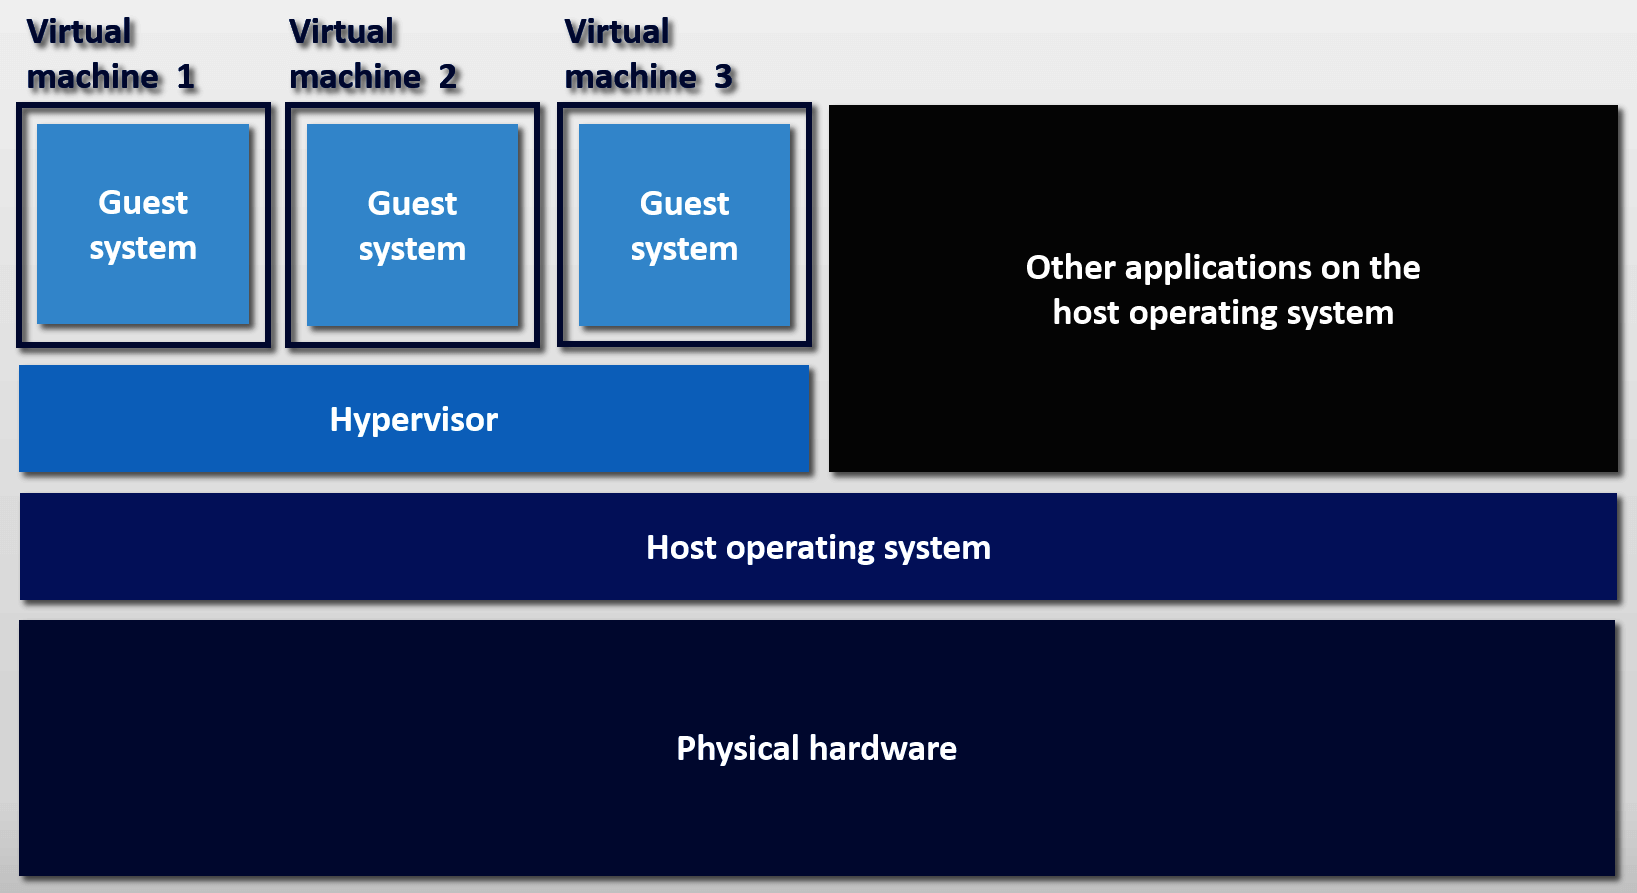
\includegraphics[width=\textwidth]{img/vm-1.png}
    \caption{Operating system view if there are VMs in the physical machine (source: \href{https://www.ionos.co.uk/digitalguide/server/know-how/virtual-machines/}{ionos}).}
\end{figure}

\noindent
A little terminology about \emph{host} and \emph{guest}:
\begin{itemize}
    \item \textbf{\underline{Host}}: the underlying platform supporting the environment/system.
    \item \textbf{\underline{Guest}}: the software that runs in the Virtual Machine environment as the guest.
\end{itemize}

\newpage

\paragraph{Process VM}\label{Process VM}

A \definition{Process Virtual Machine}, sometimes called an application virtual machine, or Managed Runtime Environment (MRE), \textbf{runs as a normal application inside a host OS and supports a single process}. 

\highspace
The \textbf{Virtual Machine is created when that process begins and destroyed when it ends}. A good example is the Java Virtual Machine JVM (see more \href{https://en.wikipedia.org/wiki/Java_virtual_machine}{here}).

\highspace
The purpose of a process VM is to execute a computer program in a platform-independent environment, meaning it can run on a variety of hardware or software.

\highspace
The virtualizing software:
\begin{itemize}
    \item is placed at the ABI\footnote{An \definition{Application Binary Interface (ABI)} corresponds to \dquotes{\emph{Operating system machine level}}.}, on top of the OS/hardware combination.
    \item emulates both user-level instructions and operating system calls.
    \item is usually called Runtime Software.
\end{itemize}

\begin{figure}[!htp]
    \centering
    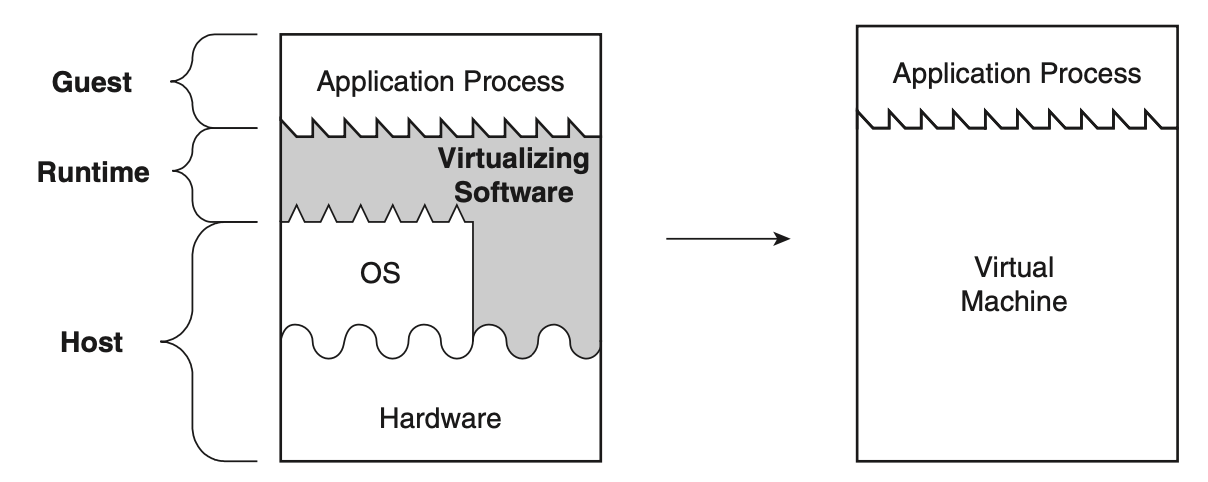
\includegraphics[width=.9\textwidth]{img/vm-2.png}
    \caption{Process VM.}
\end{figure}

\newpage

\paragraph{System VM}\label{System VM}

\definition{System Virtual Machine}s are substitutes for real machines and \textbf{provide all the functionalities of an actual operating system}. It provides operating system running in it access to underlying hardware resources (networking, I/O, GUI).

\highspace
With a system VM, the hypervisor will access the underlying machine's resources, giving the user the same capabilities the host device offers.

\highspace
The \textbf{virtualization software is called \definition{Virtual Machine Monitor (VMM)}}.

\begin{figure}[!htp]
    \centering
    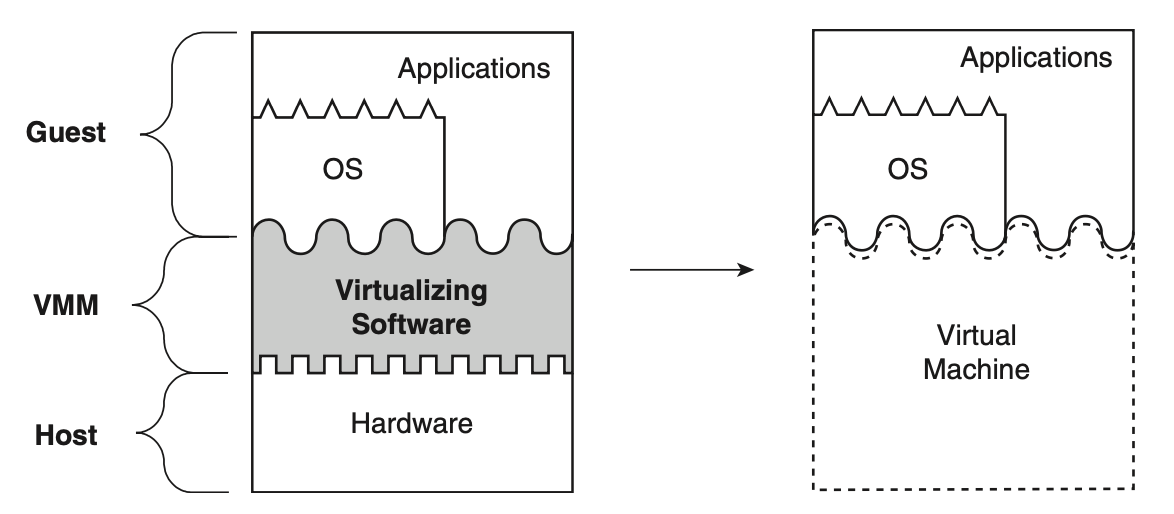
\includegraphics[width=.9\textwidth]{img/vm-3.png}
    \caption{System VM.}
\end{figure}

\newpage

\subsubsection{Virtualization Implementation}

Consider a typical layered architecture of a system by adding layers between layers of the execution stack. Depending on where the new layer is placed, we get different types of virtualization. The virtualization technologies are:
\begin{itemize}
    \item \definition{Hardware-level virtualization}. The \textbf{virtualization layer is placed between hardware and OS}. The interface seen by OS and application might be different from the physical one.
    
    \item \definition{Application-level virtualization}. The \textbf{virtualization layer is placed between the OS and some application} (e.g. JVM). It provides the same interface to the applications. The applications run in their environment, \emph{independently} from OS.
    
    \item \definition{System-level virtualization}. The \textbf{virtualization layers provides the interface of a physical machine to a secondary OS and a set of application running in it, allowing them to run on top of an existing OS}. It is placed between the system's OS and other OS (e.g. VMware, VirtualBox). We can enable several OSs to run on a single hardware.
\end{itemize}
The properties of virtualization technologies are:
\begin{itemize}
    \item \textbf{\underline{Partitioning}}
    \begin{itemize}
        \item Execution of multiple OSs on a single physical machine;
        \item Partitioning of resources between the different VMs.
    \end{itemize}
    
    \item \textbf{\underline{Isolation}}
    \begin{itemize}
        \item Fault tolerance and security (hardware level);
        \item Advanced resource control to guarantee performance (managed by the hypervisor).
    \end{itemize}
    
    \item \textbf{\underline{Encapsulation}}
    \begin{itemize}
        \item The entire state of a VM can be saved in a file (e.g. freeze and restart the execution);
        \item Because a VM is a file, can be copied/moved as a file.
    \end{itemize}
    
    \item \textbf{\underline{Hardware independence}}
    \begin{itemize}
        \item Provisioning/migration of a given VM on a given physical server.
    \end{itemize}
\end{itemize}

\newpage

\subsubsection{Virtual Machine Managers (VMM)}\label{subsubsection: Virtual Machine Managers (VMM)}

\paragraph{Paravirtualization}

\paragraph{Full virtualization}

\paragraph{Containers}
